\section{Implementation}
\label{sec:Implementation}

This section describes the key implementation details to support state capture of Python programs in River.  We explain the essentials of virtual resource (VR) execution in River and how we decouple VR state from the rest of the River run-time system.  As previously mentioned, we rely on Stackless Python in order to save the execution state of a running Python thread.  We explain how we utilize the Stackless interface to arbitrarily preempt a running VR and capture the VR state.  In order to allow VRs to issue commands to the River run-time system, we introduce atomic {\it system calls} that prevent preemption at undesirable points in execution.  We show how blocking River system calls interact with Stackless execution.  Finally, we describe how we implement distributed checkpointing.

\subsection{River Execution}

As described in Section~\ref{sec:River}, a River program is simply a Python program with a main class that inherits from the VR class.  The River run-time system consists of a Python interpreter and River VM support code.  The resulting execution environment consists of three Python threads: a network thread, a control VR, and the application VR (see Figure~\ref{fig:river-vm}). 

\begin{figure}[htb]
\centering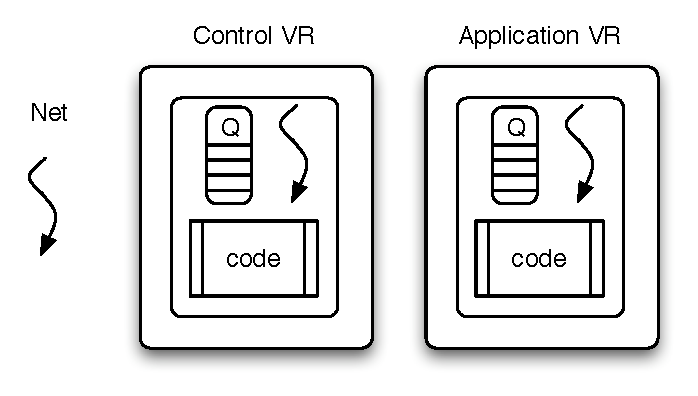
\epsfig{file=river-vm.eps,width=2.5in}
\caption{River VM Execution}\label{fig:river-vm}
\end{figure}

The network thread is used to manage socket-based communication with other River VMs.  The network thread multiplexes connections using the Python \verb+select()+ OS call.  It can handle TCP connections as well as UDP packets for multicast support.  On receipt of a packet, the network thread converts the serialized byte stream to a River message object instance, which is placed in the proper destination VR queue.  The control VR is a special VR that can perform tasks such as allocation and deployment.  The control VR can be extended to handle remote console access and to respond to state control requests.

Application VRs can be specified for launch on the command line or they can be deployed by existing VRs.  While River supports multiple application VRs per River VM, by convention we only run one application VR per River VM because Python does not support true parallel execution of OS threads.

\subsection{Using Stackless Python}

Our state management mechanism utilizes Stackless Python~\cite{Tismer:2000:StacklessPython,Stackless:2007} to capture the arbitrary run-time state of VRs.  As explained in Section~\ref{sec:StacklessPython}, Stackless Python removes the use of the C run-time stack from program execution in the Python interpreter.  This feature combined with the notion of {\it tasklets}, allows dynamic program state to be pickled just as any other Python object instance.  River state management can capture any program that utilizes standard data types and any class that can be pickled.  Exceptions include the array data type and many Python libraries that are wrappers for C libraries.

\subsection{Tasklets and Decoupling VR State}

River can run both on standard CPython and on Stackless Python. Early
implementations existed only for CPython. When running on CPython,
application VRs are executed in the context of a Python thread, which is
mapped to an OS thread. When running River on Stackless Python, the
application VR is executed as a tasklet, which, in turn, is executed in
the context of a Python thread. The host Python thread is referred to as
the {\it main tasklet}. This strategy allows us to control the execution
of the application VR.  

%We can tell Stackless to run a tasklet for a
%given number of Python instructions. After the specified number of
%instructions has executed, control is returned to the main thread. Such
%preemption can be used to see if we should stop execution in order to
%capture the execution state.  

%\begin{figure}[htb]
\begin{listing}
\scriptsize
\begin{verbatim}


self.vr.t = stackless.tasklet(self.vr.main)()

while stackless.getruncount() > 1:
  self.vr.t = stackless.run(1000)
  if self.peek(type='__state__'):
    m = self.recv(type='__state__')
    # Process state messages 'pause' and 'snapshot'
    ...
  if self.vr.t:
    self.vr.t.insert()
  else:
    break
\end{verbatim}
\normalsize
\caption{Executing a VR Tasklet}
\label{ex:vrtasklet}
\end{listing}
%\end{figure}

The code in Listing~\ref{ex:vrtasklet} shows a simplified version of the
main VR tasklet control loop in River.  The key to supporting asynchronous
checkpointing is the ability to preempt the executing VR tasklet.  This
achieved with the \verb+stackless.run(1000)+ method; it tells the
interpreter to execute a specified number of Python bytecodes.  The return
value of \verb+stackless.run()+ is the tasklet that was preempted or finished.  In our case, this will always be the application VR tasklet.  At this point we can see if the VR has received any control messages, such as a {\it pause} request or a {\it snapshot} request.

Running the application VR as a tasklet, then attempting to save
the VR state does not work without careful handling. Notice that the
tasklet is an attribute of the VR object instance. So, to serialize the
VR plus the tasklet, we need to simply pickle the VR instance. The
problem is that when the VR is pickled, the system attempts to
serialize entire state of the VR, the tasklet, and any state {\it
reachable} by these objects. However, the methods provided by the base VR
class have references and make calls into the River VM objects. Because
these objects are reachable through the VR object, serialization results
in an attempt to serialize the entire River VM run-time system.

\begin{figure}[htb]
\centering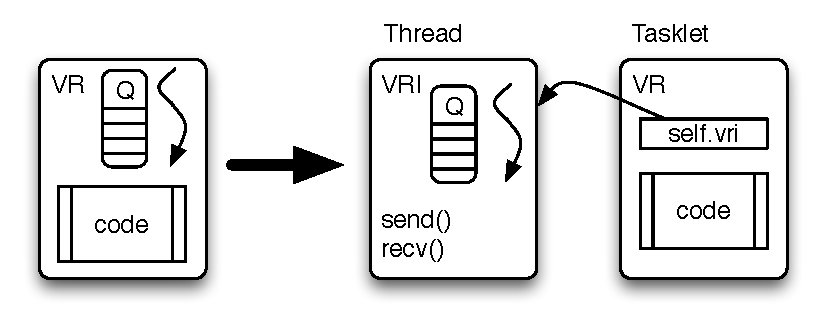
\epsfig{file=river-decoupled-vr.eps,width=3.0in}
\caption{Decoupling VR State}\label{fig:river-decoupled-vr}
\end{figure}

In order to support the serialization of just the application VR state,
we introduce the notion of an {\it internal} VR object, called VRI. The
VRI class contains all of the hard references previously contained in
the VR. Now, only the application supplied state is contained in the VR
object. However, during VR execution we create references to important
{\it system call} methods such as \verb+send()+ and \verb+recv()+. The
references are handled via a single VRI reference (See
Figure~\ref{fig:river-decoupled-vr}). By decoupling system supplied VR
state from application supplied state, we can easily {\it unlink} the
VRI reference when we need to checkpoint the VR.

\subsection{River System Calls}

The base VR class provides methods to discover and allocate remote River VMs as well as to send and receive messages among VR instances.  These methods are implemented in terms of lower-level River VM classes.  We call such methods River {\it system calls} because they require access to the internals of the River run-time system.   While the River system calls do not cross a protection boundary like conventional OS system calls, they do cross a  {\it reference} boundary that introduces River VM runtime references into the call stack of the application VR.  As such, we need to make sure that we do not try to snapshot the state of a VR while it is in the middle of a River system call.

To avoid this River VM reference entanglement, we make all River VM system calls {\it atomic} relative to \verb+stackless.run()+ preemption.
Stackless Python provides an interface to prevent such preemption via the \verb+set_atomic(value)+ tasklet method.  This allows the current tasklet to turn off preemption (\verb+value = True+) or turn it on (\verb+value = False+).  The return value of \verb+set_atomic()+ is the previous atomic state, which allows for recursive atomic sections.

System call atomicity solves one of the problems with preventing
entanglement, but the system calls themselves can introduce references from
the VR object into the River VM.  Therefore, the system calls need to be
{\it soft} references that can be created when we start or resume a VR and
unlinked when we need to snapshot a VR.  We provide system call atomicity
and soft references using Python closures.  For each system call we create
a VR method that points to a closure that performs system calls atomically and ensure that after the atomic operation there are no links from the VR back to the River VM.  

%\begin{figure}[htb]
\begin{listing}
\scriptsize
\begin{verbatim}


def gensyscall_state(self, name):
  def newsyscall(*args, **kwargs):
    t = stackless.current
    curatomic = t.set_atomic( True )
    sysmethod = self.syscalls[name]
    rv = sysmethod(*args, **kwargs)
    del sysmethod
    t.set_atomic( curatomic )
    return rv
  return newsyscall
\end{verbatim}
\normalsize
\caption{System Call Generator}
\label{ex:systemcallgenerator}
\end{listing}
%\end{figure}

The code given in Listing~\ref{ex:systemcallgenerator} is called for
each River system call (e.g., \verb+send()+, \verb+recv()+,
\verb+peek()+, \verb+discover()+, etc.). An important aspect of this code is that the system call is looked up by name in a \verb+syscalls+ table to get a reference.  This allows the system call table to be deleted just before a snapshot is taken.  When a saved VR is restored, we need to populate the system call table just before resuming execution.   Also notice the reference is needed only for the duration of the operation.  After the system call is invoked the reference is removed from the current stack activation record.  This insight did not come immediately.  We initially assumed that the reference would be removed from the stack on return from the wrapper method.  However, it turns out that because preemption can occur between any two bytecodes, we periodically ran into the case where we had completed the system call but not yet returned from the wrapper.  So, in our final solution we do not turn preemption back on until we are certain the reference to the River VM is removed.

The last significant system call implementation issue involves blocking
calls.  Currently, the only blocking call is the \verb+recv()+ call which
blocks the VR while waiting for incoming messages.  We use the same
approach described above for ensuring \verb+recv()+ is atomic relative to
\verb+stackless.run()+ preemption.  However, in order to block, the VR
message queue uses a Python Condition variable.  When new messages arrive,
the VR thread is resumed and the messages can be processed.  In order to
support asynchronous pausing and snapshots, we created special
\verb+__state__+ messages that can only be created by the system.  When the
message queue receives such a message, it returns back to the VR system call wrapper, which then yields the VR tasklet as if it had been preempted.  The VR run loop can then respond to \verb+__state__+ messages.  

\subsection{Saving and Restoring VR State}

With the assurance that the VR state will be decoupled from the VRI state (and the River VM), saving the VR execution state amounts to the following steps:

\begin{enumerate}
\item Create a state container object
\item Remove the VRI reference in the VR
\item Remove system call table (VRI references)
\item Add message queue reference to container
\item Pickle VR (includes the VR tasklet and queue)
\item Add pickled VR to container
\item Add UUID and parent UUID to container
\end{enumerate}

The resulting state container can be pickled and saved to a file or sent over the network.  Restoring the VR state on a VM works in much the same way except the state is extracted from a container and sent to a VM to be restored.

\com{
\begin{enumerate}
\item Read container file
\item Extract saved VR its UUID
\item Allocate a VR on a VM with UUID
\item Send VR state to VM (via ControlVR)
\item Create VRI thread
\item Pass in pickled VR state and queue
\item Unpickle VR state
\item Resume VR tasklet in run loop
\end{enumerate}
}%\com

One implementation detail involving Stackless Python is that tasklets are associated with the thread in which they are created.  It is possible to execute tasklets in multiple Python threads, but tasklet instances cannot move between threads.  This means that a tasklet must be pickled in the thread in which it was created.  Similarly it is necessary to run an unpickled tasklet in the thread in which it was unpickled.  If this restriction is removed in a future version of Stackless Python, it will simplify the River implementation and avoid some extra object copying.

\subsection{Internal State Capture}

Supporting the internal state capture interface amounts to a VR sending a
\verb+__state__+ message to itself.  On receipt of the message, control is
returned to the run loop and the VR state can be saved or, if specified,
the \verb+state_handler+ function can be invoked.  The VR tasklet run loop
will return to executing the VR or exit the VR as specified in the
\verb+__state__+ message.  Similarly, the VM can also be exited if desired,
in which case the VR sends an exit request to the Control VR on the VM.

\subsection{Distributed State Capture}

The external interface for distributed state capture allows an external VR to send control messages to running VRs.  The control messages are sent to the Control VR running on each VM.  The Control VR responds to the following state messages:

\begin{itemize}
\item {\bf pause} Stop the running VR
\item {\bf resume} Continue VR execution
\item {\bf getvr} Retrieve the pickled VR state
\item {\bf deploy} Start a new or saved VR
\item {\bf balance\_counts} Retrieve message counts
\item {\bf balance\_clear} Clear message counts
\end{itemize}

These control messages can be used to implement full distributed
application state capture and full or partial VR migration.  To capture the
entire distributed state we can write a utility VR as outlined in
Section~\ref{sec:ExternalInterface}.  First, we pause all VRs associated
with the application.  Second, we allow in-transit messages to settle.  We
ensure that all messages have reached their destination VRs by querying the
message counts on each VM through the {\bf balance\_counts} control
message.  Full or partial migration can be achieved by pausing all VRs,
balancing messages, then moving the desired VRs.

